\subsection{Parallel Simulation}

% The good
\subsubsection{Queue}
\paragraph*{Allocation}
The Queue model is one single chain of models. Each kernel gets one connected part of this chain. The result is that the kernels themselves also form a chain where events only travel in one direction.

\paragraph*{Strong and Weak Scaling}
Figure~\ref{fig:Queue_plot_strong} shows the speedup compared to dxex sequential for a fixed problem size.
As the amount of kernels increases, the optimistic kernel quickly becomes the worst choice.
The difference between dxex conservative and adevs becoming smaller.
The same effect can be seen for weak scaling in Figure~\ref{fig:Queue_plot_weak}.

%In Figure \ref{fig:Queue_allocation} the allocation of the Queue model is visualized. This trace allows us to demonstrate the benchmark results and explain why optimistic is not ideal for such a chain topology as present in Queue. Kernel 2 is dependent on events from kernels 0 and 1 but by definition of the optimistic synchronization protocol it will simulate ahead without waiting for events it depends on. Any simulation it performs will have to be reverted as soon as events from kernels 0 and 1 arrive. When kernel 2 reverts, kernel 3 will inevitably have to revert as well since most of the events it received from kernel 2 are invalidated and marked as such by antimessages. This leads to severe performance degradation, with an increasing probability of cascading reverts as the number of kernels and models per kernels increases.
The speedup of adevs is always in comparison with the runtime of the corresponding dxex sequential benchmark.
\begin{figure}
	\center
	
	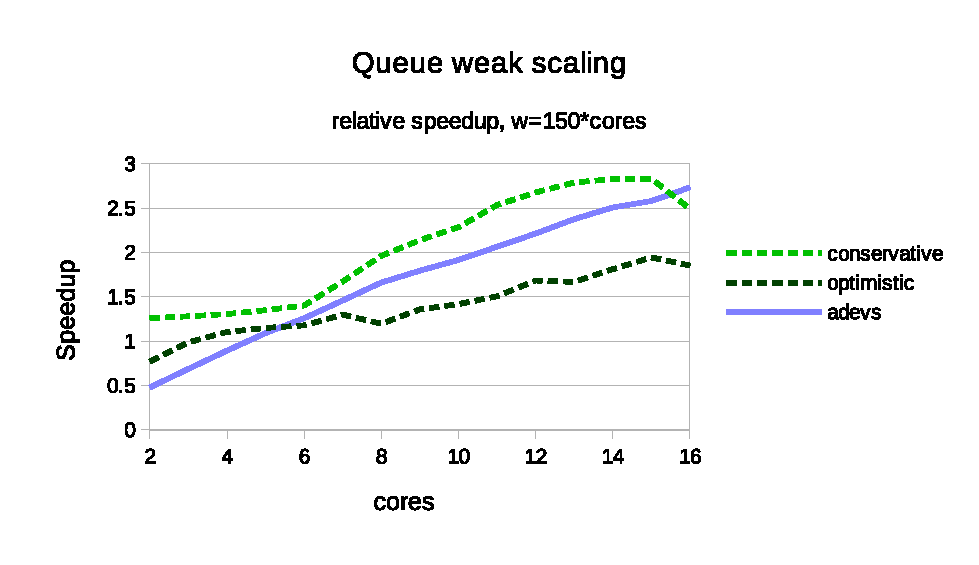
\includegraphics[width=\modelfraction\columnwidth]{fig/queue_fixed_weak_speedup.eps}
	\caption{Queue model weak scaling speedup compared to dxex sequential.}
	\label{fig:Queue_plot_weak}
	
	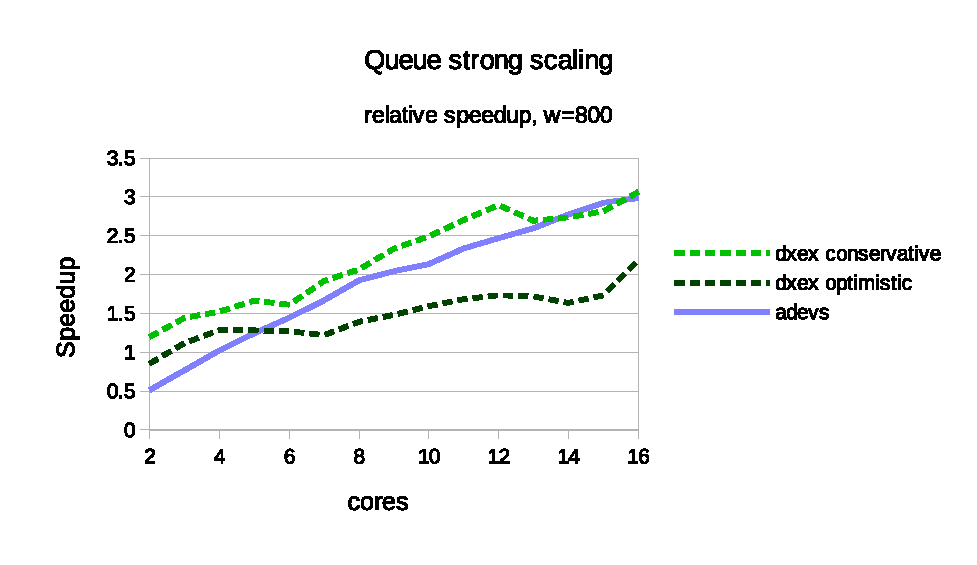
\includegraphics[width=\modelfraction\columnwidth]{fig/queue_fixed_strong_speedup.eps}
	\caption{Queue model strong scaling speedup compared to dxex sequential.}
	\label{fig:Queue_plot_strong}
		
\end{figure}

% The really bad
\subsubsection{Interconnect}\label{subsec:parallelinterconnect}
In the Interconnect model, we determine how broadcast communication is supported across multiple nodes.
The number of models is now kept constant at eight.
Results are shown in Figure~\ref{fig:interconnect_benchmark_parallel}.
When the number of nodes increases, performance decreases due to increasing contention in conservative simulation and an increasing number of of rollbacks in optimistic simulation.
All models depend on each other and have no computational load whatsoever, negating any possible performance gain by executing the simulation in parallel.
In Interconnect there is no allocation scheme possible that avoids cyclic dependencies between simulation kernels, as shown in the trace \ref{fig:interconnect_allocation_parallel} of a simulation with 4 models. Such a cycle forces sequential operation of the kernels with no speedup possible.

\begin{figure}
	\center
	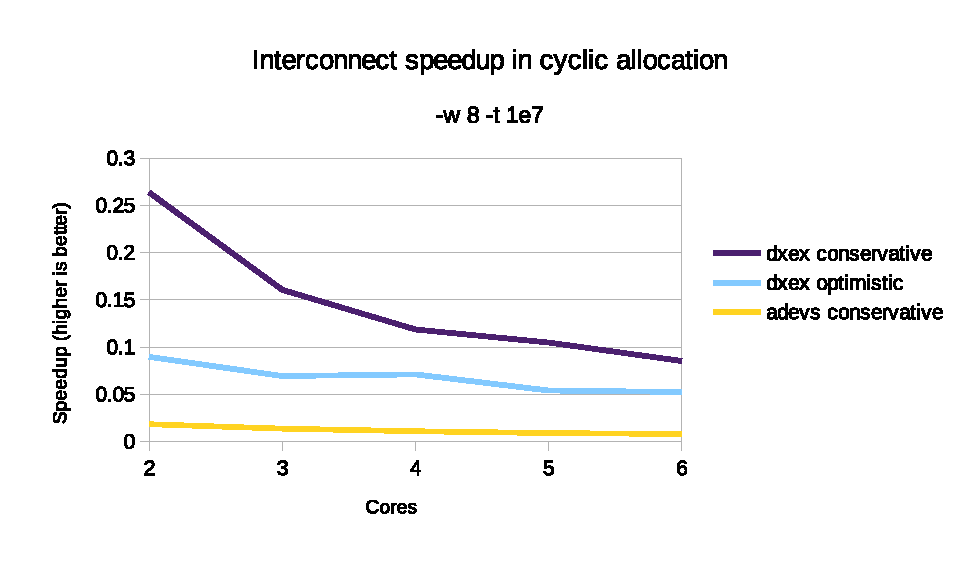
\includegraphics[width=\plotfraction\columnwidth]{fig/interconnect_parallel.eps}
	\caption{Interconnect benchmark results for parallel simulation.}
	\label{fig:interconnect_benchmark_parallel}
\end{figure}
\begin{figure}
	\center
	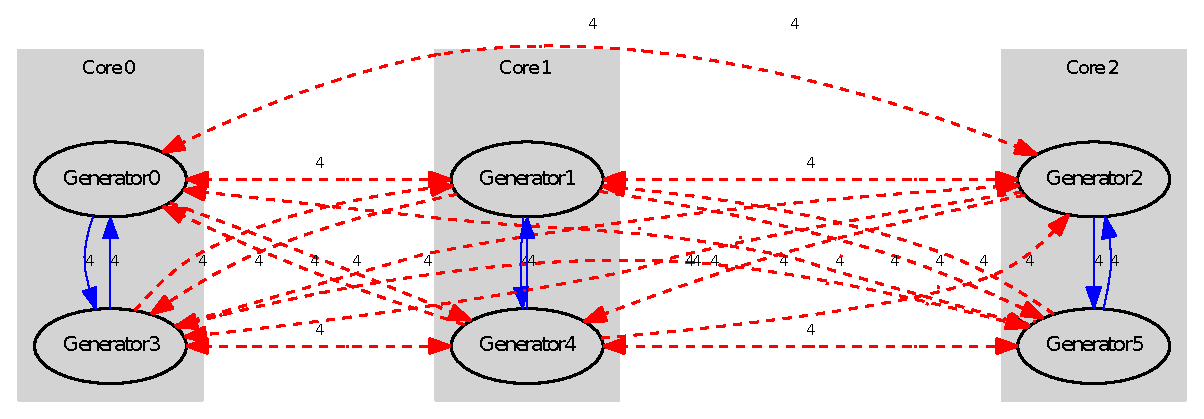
\includegraphics[width=\plotfraction\columnwidth]{fig/interconnect_parallel_allocation.eps}
	\caption{Interconnect parallel simulation trace for 6 models on 3 kernels.}
	\label{fig:interconnect_allocation_parallel}
\end{figure}

% The okayish
\subsubsection{Phold}
% Same cause, different results
In the Phold model, we first investigate the influence of the percentage of remote events on the speedup. A remote event in this context is an event that is sent from a model on one kernel to a model on another simulation kernel.
When remote events are rare, optimistic synchronization rarely has to roll back, thus increasing performance.
With more common remote events, however, optimistic synchronization quickly slows down due to frequent rollbacks.
Conservative synchronization, on the other hand, is mostly unconcerned with the number of remote events: the mere fact that a remote event can happen, causes it to block and wait.
Even though a single synchronization protocol is always ideal in this case, it already shows that different synchronization protocols respond differently to a changing model.
Adevs is significantly slower during conservative synchronization.
Analysis of profiling callgraphs shows that exception handling in adevs is the main cause. 
To keep the models equivalent, the adevs version does not provide the \{begin,end\}Lookahead methods, which accounts for the exception handling. These functions require the user to implement a state saving in contrast to PythonPDEVS and dxex's optimistic kernels which handle this inside the kernel. We feel this would lead to an unfair comparison as we would like to keep the models synchronization-agnostic across all benchmarks.

\begin{figure}
    \center
    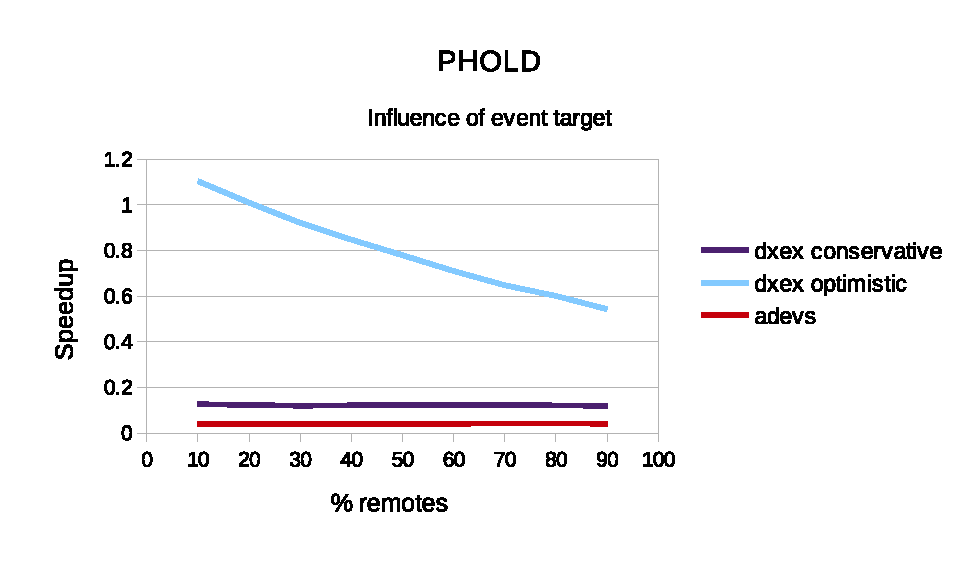
\includegraphics[width=\plotfraction\columnwidth]{fig/phold_remotes.eps}
    \caption{Phold benchmark results for parallel simulation using four kernels, four atomics per node, with varying percentage of remote events.}
\end{figure}
\begin{figure}
	\center
	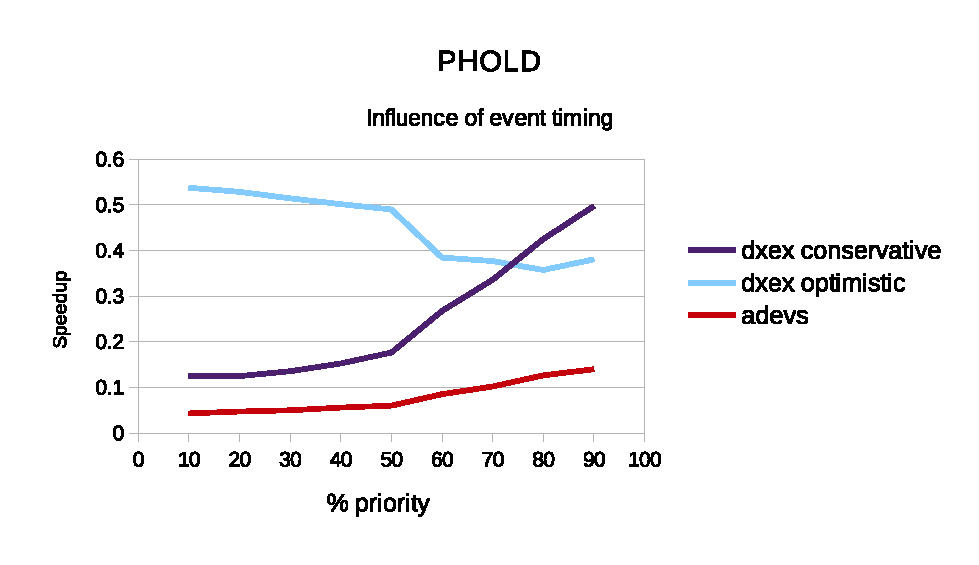
\includegraphics[width=\plotfraction\columnwidth]{fig/phold_priority.eps}
	\caption{Phold benchmark results for parallel simulation using four kernels, with varying amount of high-priority events.}
	\label{fig:phold_priority}
\end{figure}

We slightly modified the Phold benchmark, to include high-priority events.
Contrary to normal events, high-priority events happen almost instantaneously, restricting lookahead to a very small value.
Even when normal events occur most often, conservative synchronization always blocks until it can make guarantees.
Optimistic synchronization, however, simply goes forward in simulation time and rolls back when these high-priority events happen.
This situation closely mimics the case made in the comparison between both synchronization algorithms by~\cite{FujimotoBook}.
In Figure \ref{fig:phold_allocation} it is clear that in Phold it is possible for dependency cycles to form between kernels which as we have shown in Interconnect degrades performance for both optimistic and conservative. This is also the cause of the sublinear speedup observed in our Phold benchmark.

Figure~\ref{fig:phold_priority} shows how simulation performance is influenced by the fraction of these high-priority events.
If barely any high-priority events occur, conservative synchronization is penalized due to its excessive blocking, which often turned out to be unnecessary.
When many high-priority events occur, optimistic synchronization is penalized due to its mindless progression of simulation, which frequently needs to be rolled back.
Results show that there is no single perfect synchronization algorithm for this model: depending on configuration, either synchronization protocol might be better.
